\documentclass[a4j]{jsarticle} %jsrticleでもいい
\usepackage{fancyhdr} %ヘッダーを表示させるのに必要
\usepackage{listingsutf8}%日本語
\usepackage{color}
\usepackage{comment} %複数行のコメントアウトのパッケージ
\usepackage{amsmath,amssymb}
\usepackage[dvipdfmx]{graphicx}
\usepackage{here}
\usepackage{ascmac}
\usepackage{subfigure}%画像を横に配置
\usepackage{fancybox}
\setlength{\parindent}{0pt}
\setlength{\oddsidemargin}{0mm}
\setlength{\textwidth}{170mm} 
\setlength{\topmargin}{-5mm}
\setlength{\textheight}{240mm}
\setlength{\columnsep}{8mm}

\begin{comment}

\pagestyle{fancy}
  \lhead{メディア情報学プログラミング演習} %ヘッダー左
  \rhead{J1-26} %ヘッダー右
\topmargin =-15mm %ページ上部の隙間の調整

\title{令和6年度 メディア情報学プログラミング演習\\グループプログラミング レポート\\料理提供ゲーム「MiniCook」}
\renewcommand{\lstlistingname}{コード}
\begin{document}
\maketitle

\begin{center}%中央に表書く
  \begin{tabular}{|c|c|}
      \hline
      学科&情報理工学域\\
      \hline
      クラス&J1\\
      \hline
      グループ番号&26\\
      \hline
      2210259&米谷\ 祐希\\
      \hline
      2210730&鈴木\ 早紀\\
      \hline
      2210743&吉田\ 陽音\\
      \hline
  \end{tabular}
\end{center}
\end{comment}
\pagestyle{fancy}
  \lhead{メディア情報学プログラミング演習} %ヘッダー左
  \rhead{J1-26} %ヘッダー右
\topmargin =-15mm %ページ上部の隙間の調整
\begin {document}
\thispagestyle{empty}
\begin{flushright}
\begin{tabular}{|c|}\hline
\hspace*{2cm} \\
\hspace*{2cm} \\
\hspace*{1.7cm} \\ \hline
\end{tabular}\\
{\huge\tt 2025-後学期}
\end{flushright}
\begin{center}
\begin{Huge}
{\bf 令和6年度メディア情報学プログラミング演習}\\
\vspace{0.5cm}
{\bf グループプログラミング レポート}\\
\vspace{1.5cm}
{\bf 料理提供ゲーム「MiniCook」}\\
\vspace{5cm}

\begin{tabular}{|c|c|}\hline
学科&情報理工学域\\ \hline
クラス&  J1    \\ \hline
グループ番号& 26 \\ \hline
2210259& 米谷 祐希 \\ \hline
2210730& 鈴木 早紀 \\ \hline
2210743& 吉田 陽音 \\ \hline
\end{tabular}
\end{Huge}
\end{center}





\newpage

\section{概要説明}
 このゲームは、レストランで働くプレイヤーが、制限時間内に料理を作るゲームである。以下の料理提供までの手順を繰り返すことでポイントを獲得し、制限時間終了時にスコアとランクが表示される。
\begin{enumerate}
  \item オーダーの確認\par
   まず、画面上部にランダムにオーダーが提示される。オーダーには、使う食材と調理方法が記載されている。各オーダーにはそれぞれ制限時間が設定されており、残り時間はオーダー上のゲージにリアルタイムに表示される。
  \item 食材の調理\par
   次に、オーダーに記載されている食材を、各食材ボックスから取り出す。各食材を持ったまま、各調理器具の前でアクションボタンを押すことで、食材が加工される。
  \item 料理の完成と提供\par
   料理は、加工された食材とお皿を組み合わせることで完成する。それらを組み合わせて料理ができあがれば、提供口に置くことで提供となり、オーダーと一致しているか判定される。一致していれば加点、間違っていれば減点となる。   
\end{enumerate}
 また、ゲームは3画面に分かれており、スタート画面、ゲーム画面、リザルト画面がある。また、各画面や各動作にはBGMや効果音がついている。操作はキーボードのW,A,S,D,J,K,Spaceキーを用いている。\par
 作業はGitHubを用い保存・共有を行った。米谷がModelと全体の管理、鈴木がView、吉田がControllerを主に担当したが、最終的には各自の担当領域を超えて協力しながら取り組んだ。
文責:鈴木

\section{設計方針}
 図1にクラス図を示す。%%%%%%%%%%%%%%%%%%%%%%%%%%%%%
\begin{figure}[H]
  \begin{center}
  
\includegraphics[width = 135mm]{img/class_graph.png}
  \caption{クラス図}
  \end{center}
\end{figure}
 クラス図に示しているように、MiniCookというクラスが大元のクラスとなっている。
その中でインスタンスとして5つのクラスを保持している。
Startクラス・Resultクラスはゲーム開始前の画面と、ゲーム終了時にスコアの表示等を行うためのクラスである。
そして設計方針について、このゲームはプレイヤーがオーダーに従って各種料理をつくる。
その中で、プレイヤーは皿や食材をいろんな座標に置くというプロセスが起きる。それに適応、そして拡張性を保つような構成にした。詳細に関しては以下で説明する。
今回のプログラムは大量生産するインスタンスが存在しないという想定を最初の構想で予測したためObserverモデルは用いずに、基本的なMVCモデルを元にして作成した。
\begin{itemize}
  \item Model\par
   DrawModelクラスでは、各種データの管理とそれに伴ったメソッドの提供をおこなった。基本的にゲームの情報は各種クラスからModelに参照されて提供する。
  Player,Gridなどの基盤にあるようなクラスはここでインスタンスを作成している。
  \item View\par
   DrawViewでは、Modelクラスより取得した情報を元に一括で描画処理を行う。
  フィールドのどの場所にどの物を描画するかの元情報をModelより取得。
  その後その情報を元に画像をViewクラスのメソッドを用いて判定して、画像を選択・描画している。
  当初の予定では、完全に2Dでゲームを作成する予定であったが、途中で擬似3Dにして立体感を出そうという構想が生まれた。
  しかしViewモデルで一括で管理しているおかげで、プログラムの書き直しは最低限に抑えることができた。
  \item Controller\par
   DrawControllerクラスでは、基本的にはプレイヤーからの入力の受取のみを行う。
  それぞれキーボードの入力を受取、それに応じた動作をそれぞれのクラス内のメソッドでおこなってもらう。\\
   しかしゲームに動的なアニメーションを少し付ける都合でキー入力を行いたいときと行いたくないときがある。
  それに対応するために、あるクラスのメソッドを呼び出すときもあれば、キー入力中にbooleanのフラグを用いて、動作先で参照してもらう形になっているものもある。
  \item Player・Grid\par
   この2つのクラスは、このプログラムのいちばん重要なクラスである。
  名称が違うもののプレイヤーが食材を保持している場合とあるマス目が食材を持っている(食材を置いている)という違いがあるのみで、ほとんど同じものである。
  このクラスでは、そのマスないしはプレイヤーがなにを持っているかというクラスをインスタンス変数に保持している。そして、Playerに許された行動やGrid(マス目)によってできる。
  行動についての自身の情報を持っており、それに対応したメソッドを提供している。
  \item Order\par
   Orderクラスでは、画面上部に定期的なタイミングで出現する、提供しなければならない料理の情報を持っているクラスである。
  注文1つごとにこのクラスが生成されて、その中にオーダーの制限時間、必要な材料などの情報をしている。
  \item Food\par
   このFoodクラスが、食材に関しての最小単位となるクラスである。抽象クラスという定義をしており、これを継承してキャベツであったり、トマトであったりのクラスを作成している。
  それぞれ継承されたクラスにおいて。それぞれ特有の調理される方法や、調理された情報を保持することができる。これを複数個ミックスして料理となったものが後述するPlateクラスである。
  \item Plate\par
   このPlateクラスでは、Foodクラスをいくつか保持していて、それによって例えばキャベツとトマトのサラダであったり、魚の切り身と海苔で巻き寿司といったものになる。
  これがOrderに存在していれば正解、なければ不正解という形である。
  また各マス目とPlayerはFoodクラスを単体で保持して食材を持っていたり、Plateクラスを持っていて、複数の食材からなる料理を持っていたりする。
  なお正誤判定についてはOrderクラスで行わずこちらでOrderクラスの内容をModelを経由して取得して、自分との合致があるかどうかで行っている。
\end{itemize}
 クラス間の関係と全体の参照の流れを説明する。ほどんどの基本の流れはModelクラスを参照して行われる。
ユーザーからの入力はDrawControllerからModelへ、描画はModelを参照してDrawVierクラスな内で行われる。
プレイヤーは移動をして該当の場所に移動してアクションを行うことで、Foodクラスを新たに生成したり、その場においたり、またそれらを調理してまとめてPlateクラスに保持する。
それを提出口に提出した際に、現存しているオーダーとの正誤判定を行いスコアのアップダウンを行う。ここでは説明を省略したが、各種タイミングでSEやBGMを鳴らすようなコードも含まれている。
\\文責:米谷




\section{プログラムの説明}
 以下にクラスとその説明を示す。
\begin{itemize}
  \item MiniCook\par
   このクラスでは、まず最初にMVCモデルの各種クラスを生成する。そして各種クラスの中にある、getter,setterを利用してそれぞれのクラスを連携させる。
  それに加えてオーディオの管理のクラスを生成したして、JFrameを用いてウィンドウを立ち上げる。
  \\ このインスタンスメソッドとしてスタート画面からゲームが画面に切り替えるstartGame()であったり、リザルト画面に切り替えるshowResult()というメソッド等を持っている。
  public~static~void~main()は個々で宣言がしてあるため、このゲームは java MiniCookでスタートする。
  \\文責~:~米谷
  \\
  \\
   このクラスでは、CardLayoutを用いることで、スタート画面・ゲーム画面・リザルト画面を1つのウィンドウで切り替える仕組みを実現している。
  このCardLayoutの仕組みにより、\texttt{cardLayout.show(panel, "画面名")} を呼び出すだけで、異なる画面を簡単に切り替えられる。例えば、スタート画面からゲームを開始する際には \texttt{startGame()} を呼び出し、\texttt{cardLayout.show(cardPanel, "game")} によってゲーム画面へ遷移する。また、ゲーム終了時には \texttt{showResult()} を呼び出し、スコア情報をリザルト画面に反映した上で \texttt{cardLayout.show(cardPanel, "result")} により遷移させている。

   また、ゲームの進行に応じて BGM を管理する仕組みも実装した。例えば、\texttt{restartGame()} では \texttt{audio.playBGM("./sound/music\_background2.wav")} を呼び出し、ゲーム再開時に適切なBGMを流すようになっている。

  文責:吉田

  \item Model\par
   前の章でも少し触れたが、このクラスではゲームに関する基本的なデータを持っている。
  インスタンス変数にGridクラス、Playerクラス、orderを入れる配列、制限時間を入れる変数などを持つ。
  MiniCookクラスより、自身が生成されたとき、Gridと呼ばれる各マスのついての2次元配列を作成してそれをフィールドとしている。
  コンストラクタのその後は、フィールドの壁や障害物、食材を加工できるツールますであるかという情報を、Gridの変数を変更していくことによって設定していく。
  基本的な動作はModelを経由して行われるようななっており、例えばplayerの移動は一旦Model.movePlayer()が呼ばれた後に、その中でplayer.move()を呼ぶことでカプセル化をより厳密なものにしている。
  またorderの生成を行うgenerateOrder()メソッドもここにあり、登録されている料理からランダムなものを生成して、それらのセッティングをしてオーダーを作っている。
  そのほかにも、オーダーを削除するremoveOrder()、スコアの増減に関するscoreUP(),scoreDown()などのインスタンス・メソッドを持っている。
  \\文責~:~米谷

  \item Grid\par
   Gridクラスは各マス目1マスについてのクラスである。この集合を配列に保持してModelでインスタンス変数に持ってもらう。
  今回の設計として、あるマスにがあるときはそのグリッドが食材を持っているということになっている。
  つまりGridがFoodクラスやPlateクラスのオブジェクトを持つということである。
  そしてそれに伴ったインスタンス変数を作成してそこに代入している。
  ほかにも、そのマスがツールマスであるかどうかのtool、皿が置かれているかのisPlatePlacedなどの変数も用意されている。
  このクラスでは、処理をすることがないので、getterのみのインスタンスメソッドである。
  \\文責~:~米谷

  \item Player\par
   Playerクラスは基本的なインスタンス変数についてはGridクラスと同じである。そのプレイヤーが何を持っているかの変数がある。
  それに加えてPlayerならではの変数が追加されている。プレイヤーの座標であるposX,posYや、アニメーションをつけるさいのプレイヤーが今動いているかどうかのmovingという変数、
  プレイヤーの向きを表すdirection等がある。\\
   このクラスではGridクラスに加えて、プレイヤーがすることができる各種行動に対応したメソッドが用意されている。
  \begin{itemize}
    \item move() \\
     このメソッドはプレイヤーの座標を変更する。個々では離散的に値を変化させている。
    アニメーション用の座標は別途用意されていて(viewで参照される)、それの値の変化はこの座標に滑らかに一致するようになっている。

    \item getFrontGrid() \\
     インスタンス変数のdirectionを参照して、自分が対面しているGridを渡す。

    \item action() \\
     スペースキーを押されたときに呼び出されるメソッド。
    getFrontGridより得たGridのtoolを参照して、できる行動が実行される。
    自分が持っているFood,Plateの中身に対して、食材の状態変数を変化させて食材を加工させている。

    \item pick\_up() \\
     このメソッドはキー入力"J"に対応するメソッドである。同様にfrontGridの情報を取得して、そのマスに対応して、皿を持ったり食材を拾ったりする。
    このゲームに存在する食材が無限に生成される箱の前であれば、目の前のGridから取得するのではなく、あらたにnew Food()として、新たな食材を手にもつ。
    また複数の食材を一度にもつゲーム性になっているため、ここの条件文によってその食材は一緒にもてるのか、加工されいない状態ではないのかという判定を経て、実行される。

    \item put() \\
     ものをおいたり、ものを捨てたり、ものを提供したりする関数である。frontGridの情報を取得して行う。
    pick\_up()と同様に、目の前のマスに関する情報を参照して、可能なアクションをとる、そこに食材が置いてあれば、まとめて新たな食材に変化する関数を内包している。
    特別な処理としては、カウンターに提供するというイベントが有る。
    このときは、modelにPlayerが持っているPlate(料理)の情報を渡して正誤判定をしてもらう。
    それによって後述するWaiterクラスと言う演出用のクラスを呼び出してほしいとViewに知らせる。
    持ってる食材、その状態、目の前のマスの状態に応じた条件分岐がたくさんあるので、バグが頻出したメソッドでもある。
  \end{itemize}
  文責~:~米谷

  \item Waiter \\
   このクラスは、適切な料理が提供された際に、ウェイターが取りに来る演出に用いられるクラスである。
  インスタンス変数として、そのウェイターの座標と取りに来る、変える時間(フレーム数)を書いてある。
  それに加えて、自身を描画処理をするdrawMe()というメソッドをもっていて、これはviewよりGraphics~gを受け取って、
  このメソッド内で描画をする。
  \\文責~:~米谷

  \item Food\par
   このFoodクラスは、料理の食材を表現するための抽象クラスである。インスタンス変数として、食材の状態を整数値で表現するためのfoodStatu、それぞれの調理法が可能かどうかを示すフラグであるcanCut、canHeat、食材が皿の上にあるかどうかを示すフラグisPlate、食材の名前を保持するための文字列foodNameを持つ。コンストラクタでは継承した子クラスの食材にあわせて初期化が行えるように実装している。
    

  文責:吉田
  \item Plate\par
   このPlateクラスでは、料理を置く土台となる皿を表現している。Food変数の配列を持たせて皿にのっている食材を管理すると同時に、後述するOrderの必要な食材との対応関係をとりやすくしている。
  \\ hasAnyFoodは皿に食材が1つでも乗っているかを確認するメソッドである。全ての位置が null なら false を返し、そうでない場合は true を返す。
  \\ Foodクラスの引数を皿に追加するaddメソッドでは、もし同じ名前の食材が既に乗っていた場合は追加をスキップし、さらに空いてる場所があればその場所に食材を追加、満杯であれば追加しないように実装している。
  \\ getメソッドではインデックスを指定してその食材をとってくることができる。
  \\ matchesOrderメソッドでは引数で指定したOrderクラスの注文と皿に乗っている食材およびその調理状態が一致しているかを確認する。
  \\文責:吉田
  \item Order\par
   このOrderは、料理の注文を管理するクラスである。注文の基本情報を保持するインスタンス変数として、注文の名前を文字列で管理するorderName、何個目のオーダーであるかを表すorderIndex、アニメーション用の座標を表すposAnim、subOrderPosY、subOrderPosYAnimを持つ。また、食材に関するインスタンス変数として、皿を持っているかのフラグであるhasPlate、必要な食材を表すingeredient1~3がある。さらに、注文の制限時間であるtimeLimit、注文が生成された時間を示すcreateTime、自動削除用のタイマーであるexpirationTimerをインスタンス変数として持つ。制限時間が経過した場合は、効果音を鳴らし、スコアを下げ、注文が削除される。

   コンストラクタでは注文の名前や必要な食材、制限時間を注文ごとに設定できるようになっている。

   注文の完成判定を行うisCompletedメソッドはPlateクラスのオブジェクトを引数に持つ。プレイヤーが作った料理であるplate.foodと注文の材料であるorderIngredientsを1つずつ比較して、一致していれば判定用の配列をtrueとする。全ての食材が揃っていればtrueを返す。

   残り時間を計算するメソッドとしてgetRemainingTimeがある。これは現在時刻から注文作成時刻を引くことで経過時間を計算し、timeLimitから経過時間を引くことで残り時間を取得する。

   getRemainingTimeが0以下であるかで注文の期限切れを判定するisExpiredメソッドと、手動で注文を削除する際にタイマーを停止するためのcancelTimerメソッドも用意している。

  文責:吉田
  \item View\par
   このDrawViewクラスは、JPanelを継承した、描画処理用のクラスである。ゲームの基本画面やプレイヤー、食材、ツール、オーダー、ウェイターなどを描画する。
  DrawModelを参照している。インスタンス変数としてmodel,cont,sizeなどを持つ。\par
   背景やプレイヤー、オーダー、UIなどの基本的なゲーム画面の描画についてはpaintComponentで行っている。ウェイター描画はaddWaiterで行っている。\par
   食材の描画でsetFoodImage、皿の描画でsetPlateImage,オーダーの描画でsetOederImageが用いられる。これら関数では、引数として情報を受け取ってそれに対して適切な画像を返す。その判断はif文やswitch文を用いているが、特に皿の上で食材を組み合わせた場合に、載っているべき食材を指定するだけでは、載っていないべき食材の有無に関わらず完成してしまう。そのため全ての食材の種類と加工の種類を指定しなければならないが毎行書くことは冗長で現実的ではない、ということに苦労した。
  一気に食材を指定するのではなく、まず先に共通して使っていない食材をジャンルごとに指定し、そのジャンルのif文内で、持っている物持っていない物を指定することで文章量や比較を減らした。\par
  文責:鈴木   
  \item Controller\par
   主要なクラスメンバとしてはゲームのデータモデルであるmodel、画面描画用のview、プレイヤーオブジェクトplayer、ゲームアプリケーションのmainApp、新しいオーダーを定期的に追加するためのタイマーorderTimer、ゲームの時間管理用タイマーgameTimer、スペースキーが押されているかの状態を表すspacePushingがある。

   キー入力の処理を行うkeyPressedメソッドをオーバーライドし、WASDでプレイヤーの移動、Jでアイテムを拾う、Kでアイテムを置く、SPACEでアクションを行うなどのゲームの主要な操作を実装した。

   startGameメソッドでは、model.generateOrderで最初のオーダーを生成し、orderTimerによって一定時間ごとに新しいオーダーを追加する。gameTimerで1秒ごとにゲーム時間を管理し、残り時間が10秒および0秒時に効果音を再生する。残り時間が0になったらgameTimerを停止し、リザルト画面へ移行する。

   注文管理を行うstopOrderTimerメソッドではmodel.ordersに登録された全オーダーのタイマーを停止する。さらにorderTimer.stopによって新しい注文が来ないようにしている。

  文責:吉田
  \item Start\par
   このStartクラスは、MiniCookゲームのスタート画面を作成するためのJPanelである。JPanelを拡張し、タイトルとスタートボタンを持つスタート画面を作成した。フォントを読み込んで適用することでゲームの世界観を統一し、GridBagLayoutを使用して要素をバランスよく配置している。ゲーム開始時の演出として、スタートボタンを押すと効果音が再生されるようになっている。

  文責:吉田
  \item Result\par
   このResultクラスはゲーム終了後のリザルト画面を表示するためのJPanelである。スコアの表示や、リトライ・終了ボタンを設置している。スコアの数字だけではなく、星評価も追加することで、ゲームらしいフィードバックの実現およびスコアの達成感を高める工夫をした。また、MiniCookのインスタンス変数を受け取り、リスタート処理などを呼び出せるようになっている。

  文責:吉田
  \item AudioManager\par
   このAudioManagerクラスでは、ゲームのBGMおよびSEを制御している。javax.sound.sampled パッケージを使用し、WAV形式のオーディオファイルを再生・停止できるようにしている。静的なインスタンス変数としてClipクラスのオブジェクトを持たせることで、アプリ全体で1つのBGMを管理できるようにしている。BGMにおいては、まずWAVファイルを AudioInputStream に変換し、Clip にロードし、\texttt{loop(Clip.LOOP\_CONTINUOUSLY)}
  により無限ループ再生できるように実装した。SEではスレッドの並列処理によって同時に複数のSEを再生できるようにした。具体的には\texttt{new Thread(() -> { ... }).start();}
  とすることで新しいスレッドを作成している。

  文責:吉田
\end{itemize}



\section{実行例}
\subsection*{スタート画面}
 実行すると始めにこの画面(a)が現れる。スタートボタンを押すとゲーム画面:スタート時(c)になる。
\subsection*{リザルト画面}
 ゲーム終了後はこのリザルト画面(b)になる。スコアによってランクが星の数で表される。
\subsection*{ゲーム画面:スタート時}
 スタート時の画面(c)では、食材などは何もなく、オーダーが1つ入るところから開始される。上部にはオーダー、中央にはゲーム部分、下部にはスコアと制限時間を表示している。
\subsection*{ゲーム画面:オーダー}
 画面上部のオーダー(d)では、完成品、必要な食材、加工方法、残り時間が示されている。
\subsection*{ゲーム画面:加工前}
 加工前の食材(e)をボックスから取り出す。
\subsection*{ゲーム画面:加工後}
 調理器具でアクションを行うと加工後の画像(f)に切り替わる。
\subsection*{ゲーム画面:組み合わせ}
 皿の上に各食材を載せると画像がそれに伴い完成品(g)となる。
\subsection*{ゲーム画面:提供}
 完成した料理を提供口に置くと、ウェイターが取りに来る(h)。
\newpage
\begin{figure}[H]
  \begin{center}
    \subfigure[スタート画面]{
      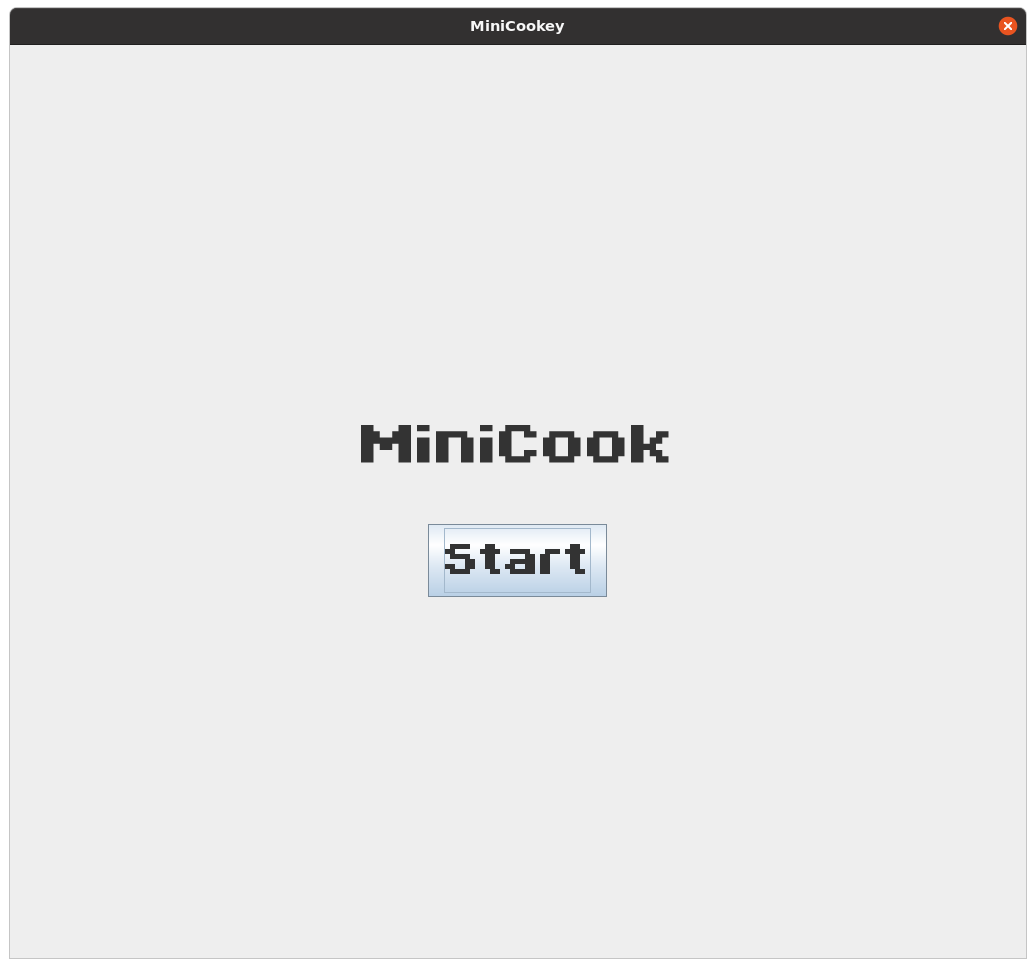
\includegraphics[width=0.4\textwidth,keepaspectratio]{img/a.png}
    }
    \subfigure[リザルト画面]{
      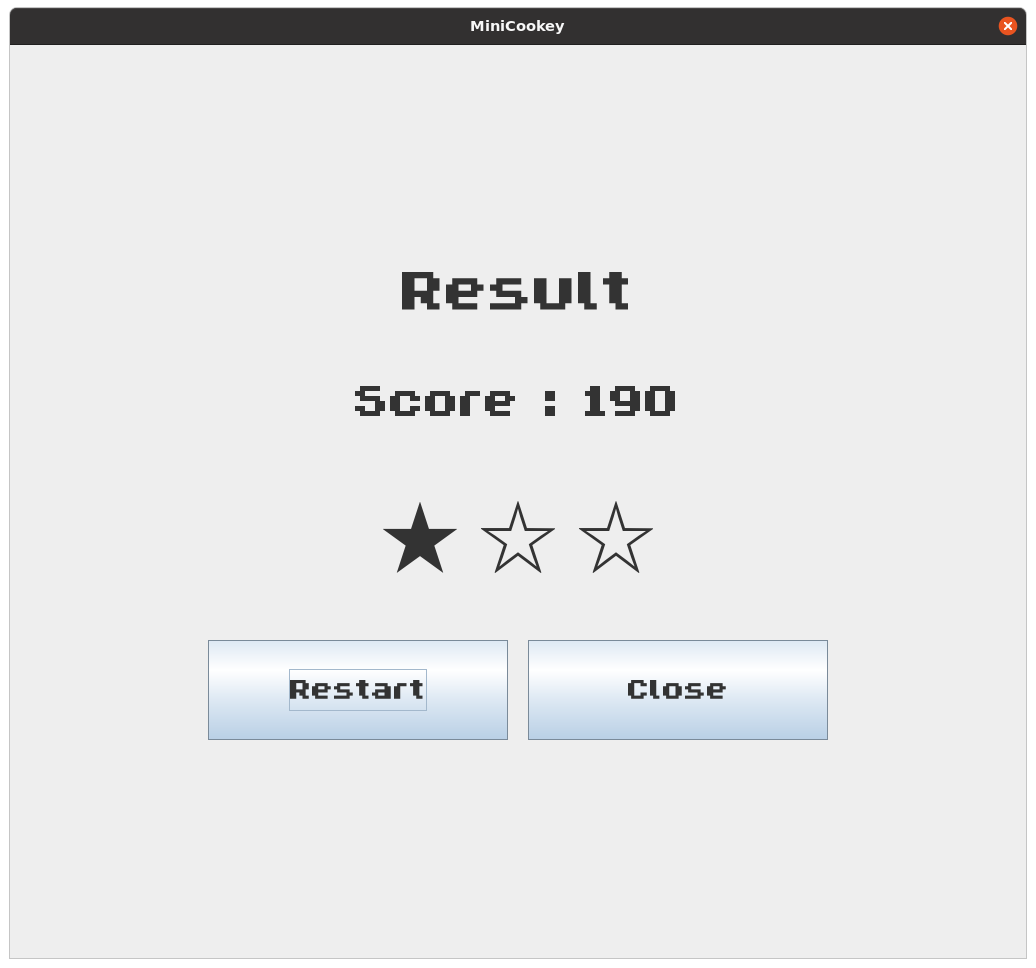
\includegraphics[width=0.4\textwidth,keepaspectratio]{img/b.png}
    }
  \end{center}
\end{figure}
\begin{figure}[H]
  \begin{center}
    \subfigure[ゲーム画面:スタート時]{
      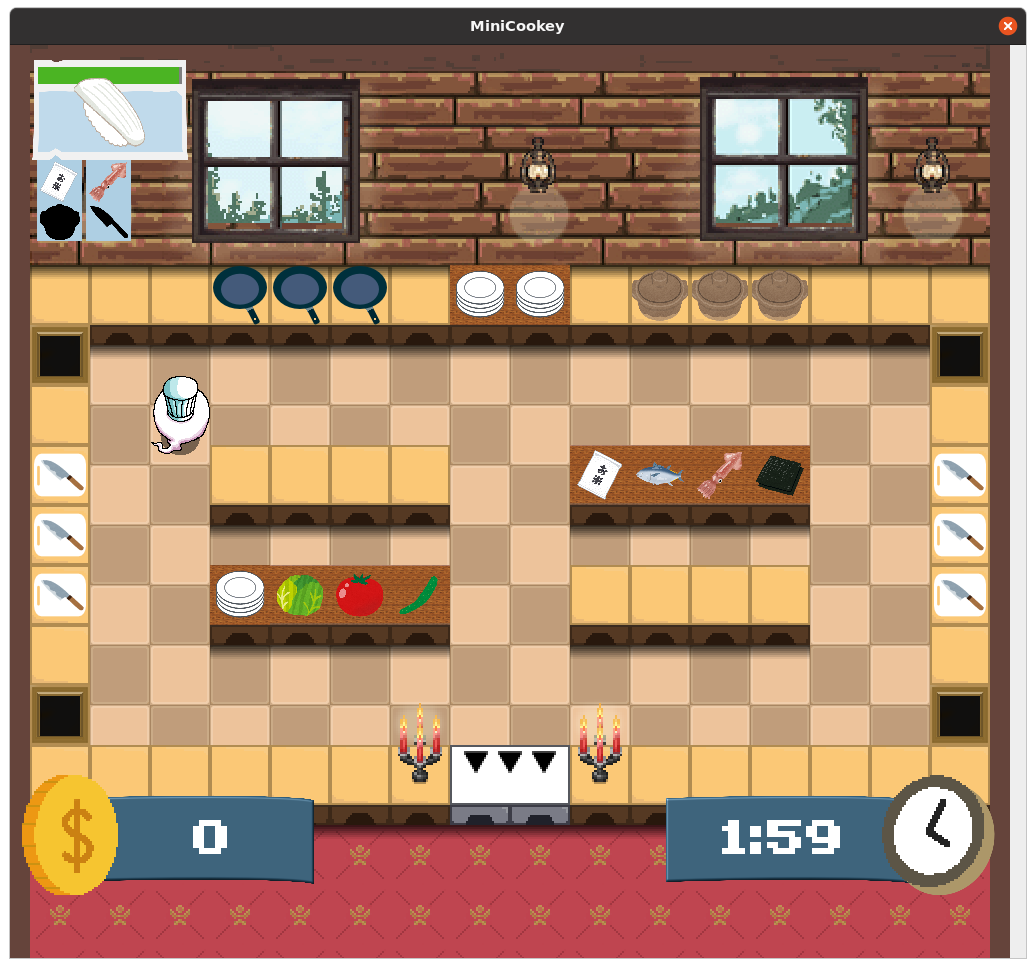
\includegraphics[width=0.4\textwidth,keepaspectratio]{img/c.png}
    }
    \subfigure[ゲーム画面:オーダー]{
      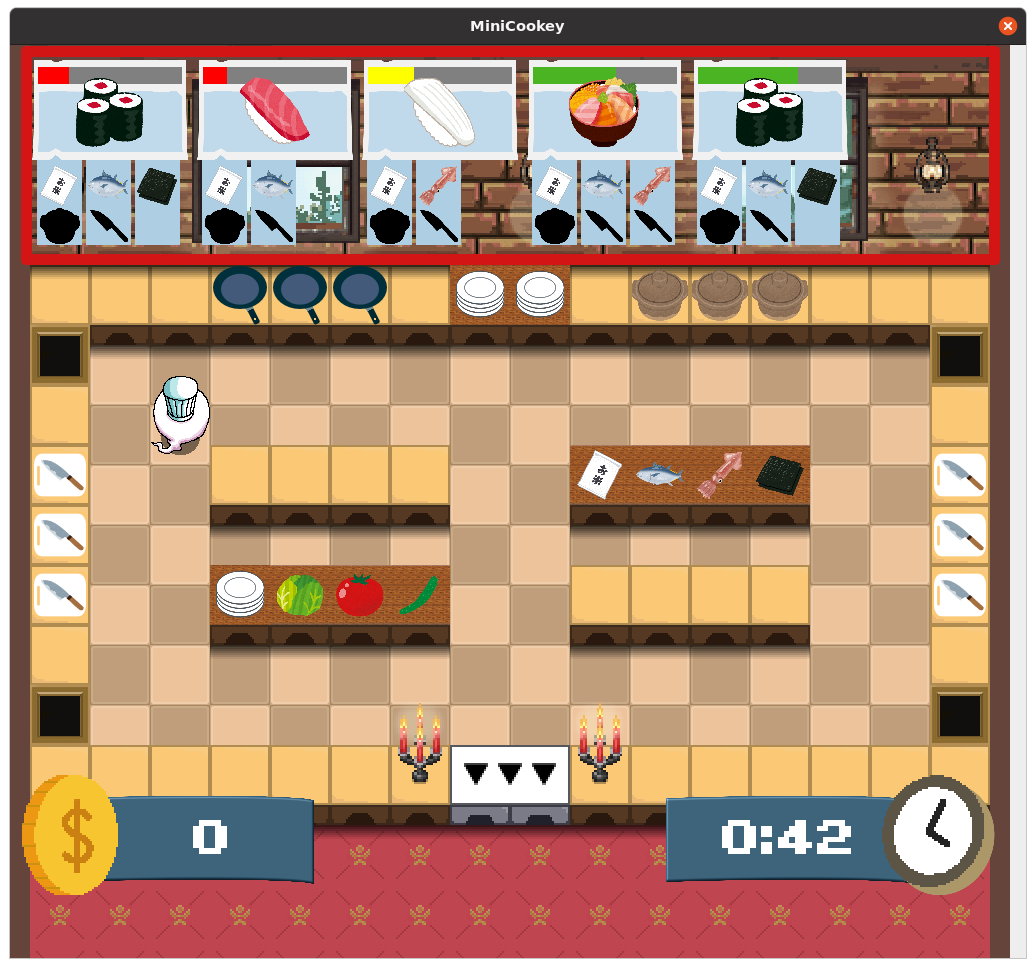
\includegraphics[width=0.4\textwidth,keepaspectratio]{img/d2.png}
    }
  \end{center}
\end{figure}
\begin{figure}[H]
  \begin{center}
    \subfigure[ゲーム画面:加工前]{
      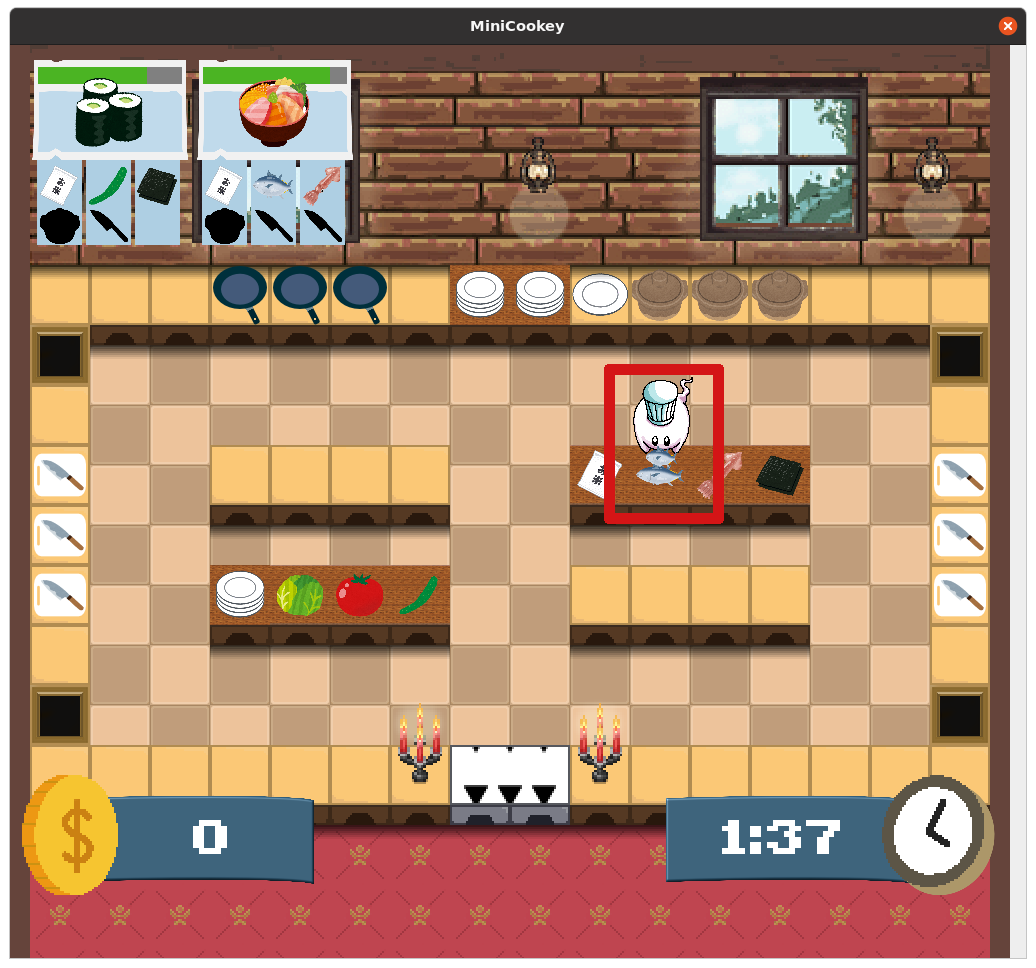
\includegraphics[width=0.4\textwidth,keepaspectratio]{img/e2.png}
    }
    \subfigure[ゲーム画面:加工後]{
      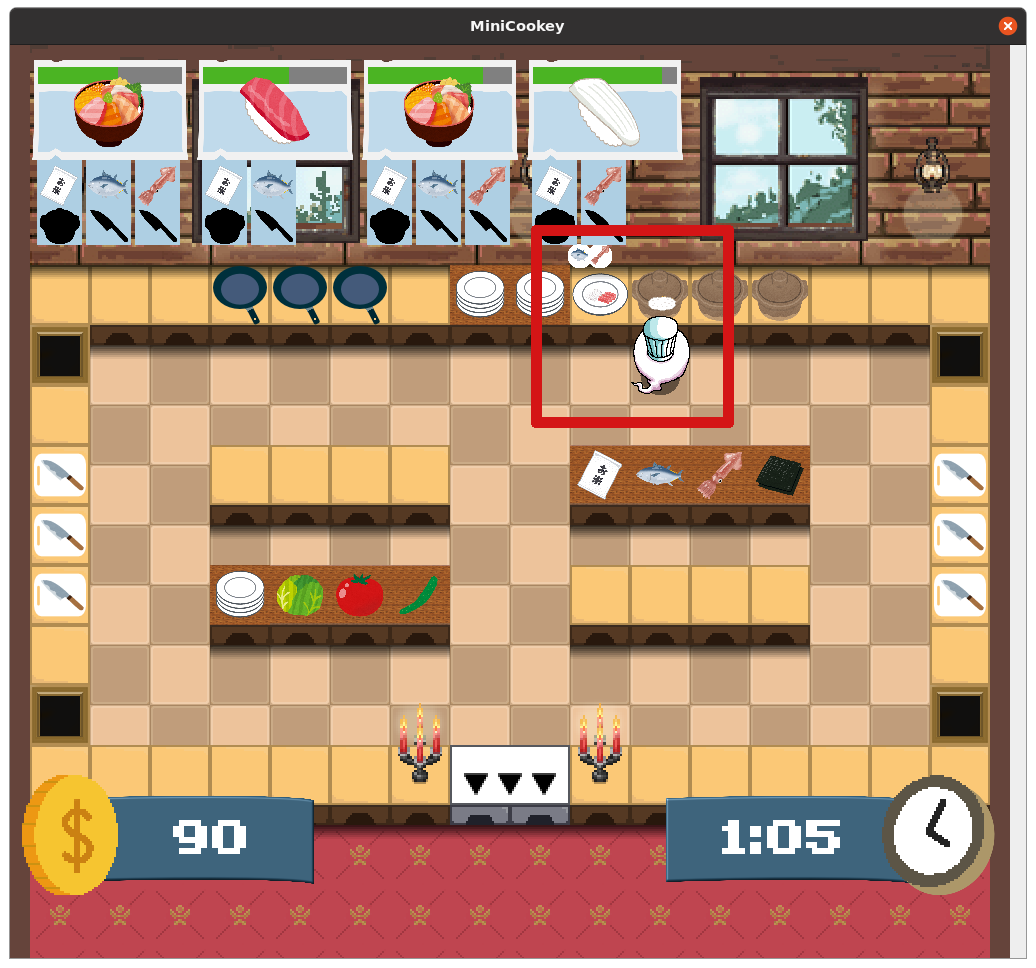
\includegraphics[width=0.4\textwidth,keepaspectratio]{img/f2.png}
    }
  \end{center}
\end{figure}
\begin{figure}[H]
  \begin{center}
    \subfigure[ゲーム画面:組み合わせ後]{
      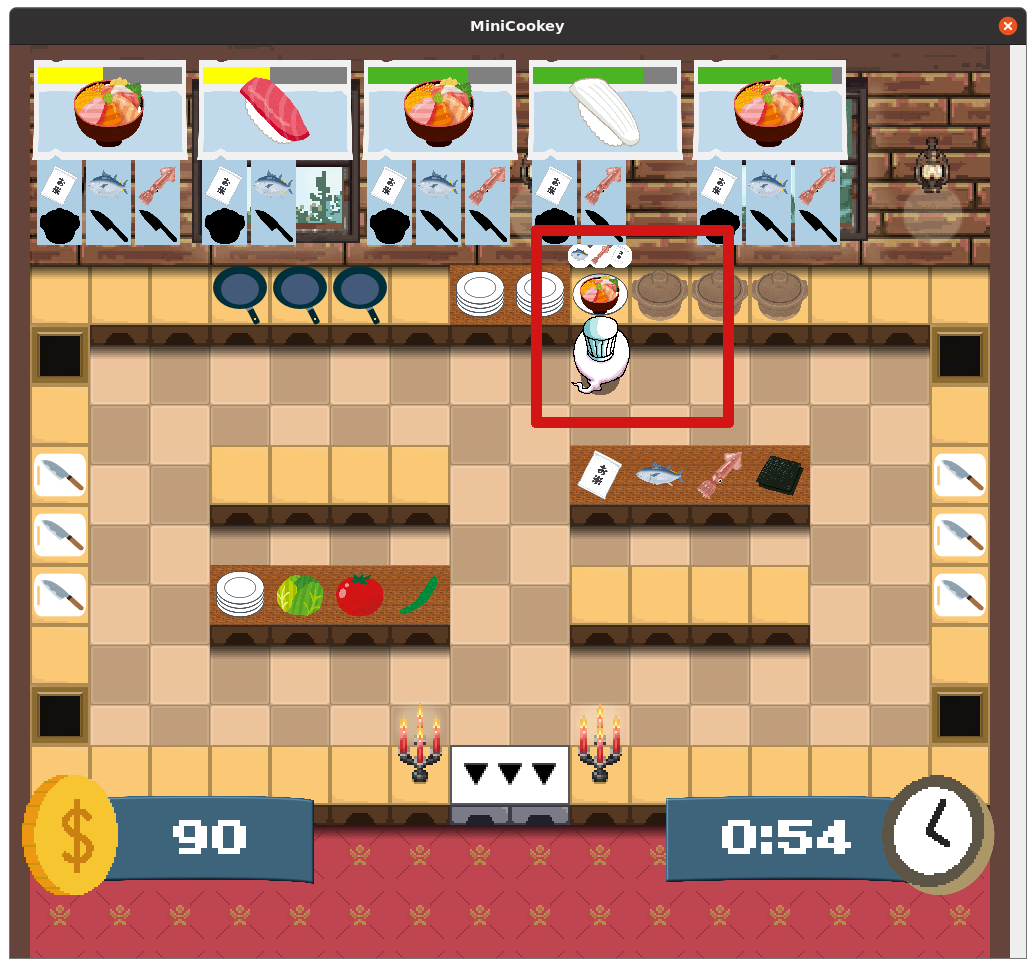
\includegraphics[width=0.4\textwidth,keepaspectratio]{img/g2.png}
    }
    \subfigure[ゲーム画面:提供]{
      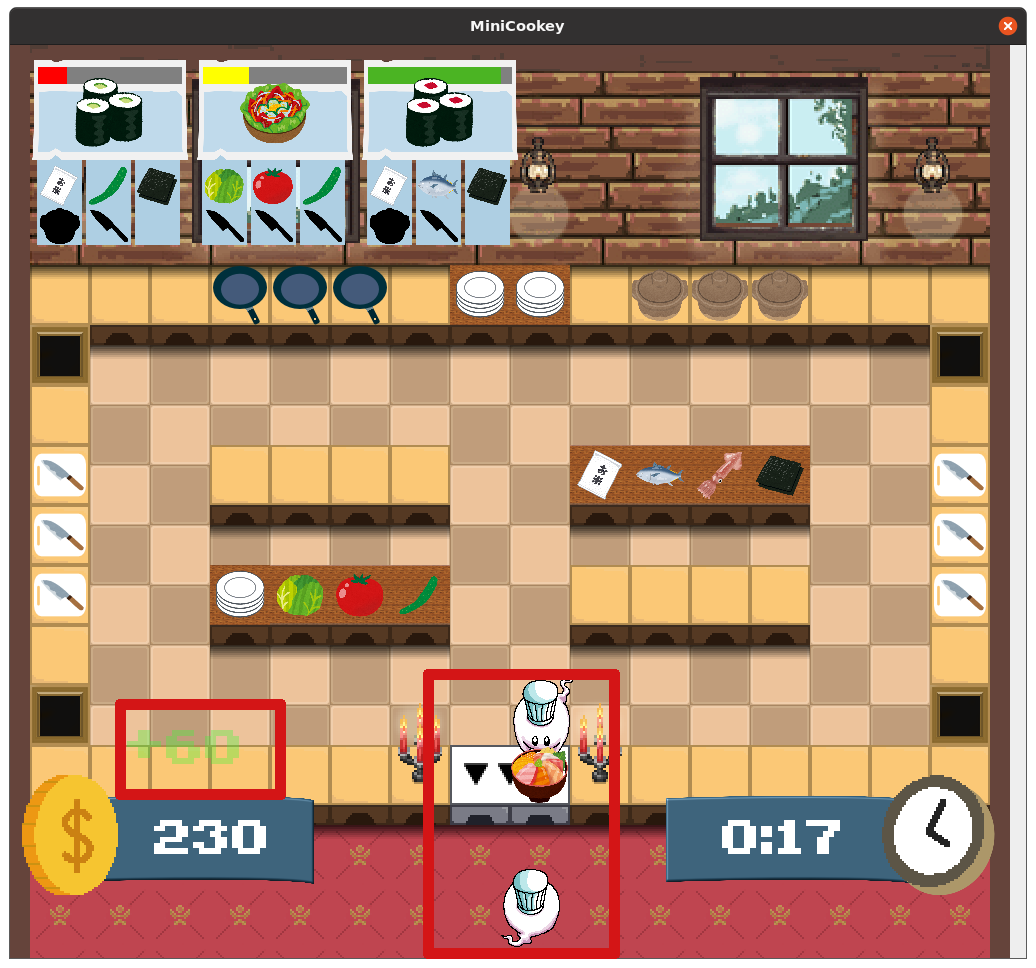
\includegraphics[width=0.4\textwidth,keepaspectratio]{img/h2.png}
    }
  \end{center}
\end{figure}
文責:鈴木

\newpage

\section{考察}
 かなり煩雑で冗長な部分を多く含むコードになっており、これは計画的な開発が行えていないことが主な理由であると考える。これは全体として大きな反省点である。
\\ PlateクラスをFoodクラスの土台として、Orderクラスと比較するという構造およびその処理はかなり直感的でありながら効果的に実装できた。
\\ Player クラスのアクションや、View のアニメーション・画像の描画処理、並びに Food クラスと Order クラスの設計は再利用性が高く、容易に拡張できるようになっている。そのため、新たな調理方法や食材、注文を追加する際にも、既存のコードやその構造を大きく変更することなく実装が可能である。このように拡張性を持たせることは、ゲームやアプリケーションの開発において重要な要素であり、本プロジェクトではその柔軟な拡張性を実現できた。

 特に、Food クラスや Order クラスでは、新しい食材や注文の種類を追加する際に、既存のコードを変更せずに新たなインスタンスを定義するだけで対応できるため、開発の負担を軽減できる。また、View の描画処理においても、新しいアニメーションや画像を追加する際に大規模な修正を加える必要がないため、デザイン面での自由度も高い。

 今後、新しい調理方法や特殊な注文の導入、さらにはマルチプレイ対応など、さらなる機能拡張を行う際にも、この柔軟な設計が活かされると考えられる。特に、追加要素が増えてもコードの可読性や保守性を損なうことなく、スムーズに機能を拡張できる点は、本プロジェクトの大きな強みである。

文責:吉田

\section{感想}
\subsection*{(米谷\ 祐希)}
 Javaを始めてさわる・オブジェクト指向言語も初めてさわる・グループ開発も初めてという、何もわからない状態で始まったのでとても大変だったというのが正直な感想です。
最初にどんなゲームを作ろうというのを全員で共有はしたものの、実際に全員が同じビジョンを見据えてコーディングをしていくというのはとても大変なのだなとつくづく実感しました。
とくに、今回全体の管理を行った関係で、チームメンバーにいろいろ指示を出すことが多かったのですが、同じ部分をそれぞれ編集するや、仕様の勘違い等で、思った通りにいかないことがあったりなど、とにかくいろんな壁がありました。
さらにクラスに関しても、これはあったほうが良いね、これもほしい、等といった付け足しの形での実装が多かったせいで、それぞれの参照などを追加したりなどという作業で一通り更新するのがとても大変でした。\\
 せっかくのグループ開発なのだからということで、GitHubを使ってみようとしましたが、最初は全員のコードを手作業でまとめていたりなど、手間取ったことが多かったです。しかしプロジェクトが進むにあたってはgit~mergeコマンドの挙動、
使用など、この授業の範疇ではない技術・知識についても習得することができたのは、とても身になったと嬉しい気持ちです。
C言語が主に触ってきた自分としては、オブジェクト指向の考え方には最初は困惑しましたが、講義とグループ開発での実践経験を経てその便利さについては十分に理解することができました。
しかしながら、このプログラムも改善ができる場所が山積みだなと思っています。自分はViewの描画の流れについても担当しているのですが、
一括で情報を取得して描画するというシステムは、クラスの参照の数が減ったりといった利点はあるものの、百行を超えるコードになってしまい、とても見にくいものとなってしまっています。
途中でそこに気づいたために自分が実装したWaiterクラスはWaiterクラス自身で自分を描画するというシステムにしてみて、view側でメソッドを一つ書くだけなのがとてもきれいで、これにすればよかったなと今になっては思っています。
ここに2つのコードを書いています。
\begin{lstlisting}[caption=このプログラムで基本的に採用されている描画処理方法]
  for(int i = 0; i < model.orders.length; i++){ //Orderの枚数によってループ処理
    if(model.orders[i] != null){
        Order order = model.orders[i];
        orderImage = setOrderImage(order);
        int targetPos = 20 + i * (orderW +5);
        double dx = targetPos - order.posAnim;
        order.posAnim += dx * easingFactor;
        g.drawImage(orderPaper, (int)order.posAnim, 15, orderW, orderH, this);
        drawGauge(g, "down", (int)(order.posAnim)+8, 22, orderW-16, 17, order.getRemainingTime()/order.timeLimit);
        g.drawImage(orderImage, 42 + (int)order.posAnim, 30, 75, 75, this);
        
    }
}
\end{lstlisting}
1つ目のプログラムは従来の手法で、それぞれの処理をviewの中にかいてあるせいで、コードが長くなってします。\\
それに対して、2つ目のプログラムはWaiterの描画である。
\begin{lstlisting}[caption=Waiterクラスで用いた描画方法]
  for(int i = 0; i < 5; i++){
    if(waiters[i] != null && waiters[i].active == true){
        waiters[i].drawMe(g, this);
    }
}
\end{lstlisting}
描画の処理はクラスに書いてあるので、個々では1行実行するだけで良くなっている。このような処理にすればよりオブジェクト指向らしく書けただろうにとおもっている。\\
 プログラムのシステム面がおおよそ出来上がったときに、「ゲームのデザインとグラフィックは大事だから!」と言って、デザインにも力を込めたいといったときに、みんながそれに賛同してより良いものにできたというのがこのプロジェクトの一番大きなターニングポイントではないかと思っている。
そして出来上がったゲームが、実際に最優秀賞を取れたというのが、自分は本当に嬉しく、とても良い経験をさせてもらったなという気持ちである。
オブジェクト指向のコーディングには慣れたつもりでいるので、これからも頑張っていきたいと思う。

\subsection*{(鈴木\ 早紀)}

 授業前半の個人の課題を最低限しか取り組まなかったために、2人よりJavaを理解していなくて2人に大変な部分を多く任せてしまいました。
2人が進んでやってくれたので感謝しています。画像・音楽の準備やメニューの追加、スライドやレポートは積極的に行えたと思います。
Viewとしての課題は、変数や画像読み込みが多すぎることで、今後食材やメニューの追加を行うときにもひたすらこれを書いていくのは厳しいと感じました。
せめて別ファイルにするなどして、View.java内はシンプルにする方が分かりやすいのかなと思いました。
また、メニューによって食材や調理方法を指定するときは、分量が少なくなるようにif文の順序に工夫はしましたが、
他の班の発表を聞き、csvファイルの読み込みにすることで管理もしやすくなるのかなと考えました。
今回初めて本格的にグループプログラミングを行ったので、共同作業をする大変さや、作業を分割する便利さを知ることができました。
先輩や2人のプログラムを特に参考にして理解を進めることができました。
Javaはこの授業で初めて触ったけれど、半年間という期間を考慮すると大きな成果が得られたなと感じます。

\subsection*{(吉田\ 陽音)}
 授業前半ではJavaの基礎知識やオブジェクト指向について学ぶことができたが、与えられた課題をこなすだけで受け身の学びであった。一方後半の、このゲーム製作では積極的にJavaについての理解を深めていくことができた。
Javaはこの授業で初めて触ったので、ゲーム製作の課題を聞いた当初はそれなりの形にできれば良いかなと思っていたが、実際に製作を進めていくうちに夢中になり、楽しみながらゲームを作ることができた。

 反省点としては、行き当たりばったりな開発となってしまい、クラスが煩雑になってしまったり、メソッドが冗長になってしまったりしたことである。もっと計画的な開発が行えていたら、他の要素を実装する時間が生まれ、より良いゲームを作れたと反省している。

 世の中に存在しているゲームに比べると簡易的なゲームであるが、素人なりにかなりの労力や知識を詰め込んだ気でいたため、友人や家族にこのゲームを見せた時にあまり良いリアクションを得られなかったことがかなりショックであった。この授業では、Javaについてだけでなく、こうした体験を通して学ぶことも多く、さらにはグループ開発を経験できたこともあり、自分にとってかなり有意義であったと実感している。

 投票で1位を獲得できたことは、自分にとって大きな達成感をもたらし、心から嬉しく思えた。


\newpage
\section*{付録1:操作マニュアル}
\subsection*{(ストーリー)}
 キミはおばけの国のレストランのキッチンで働いているぞ!制限時間内にオーダー通りの料理をたくさん作ろう!目指せ高得点!!
\subsection*{(実行方法)}
 「Java MiniCook」でゲームが開始する。
\subsection*{(操作方法)}
 このゲームはキーボードでキャラクターを操作する。図2にキー操作を示す。W,A,S,Dで上下左右を操作し、Jで取る、Kで置く、スペースキーでアクションを行う。
\begin{figure}[H]
  \begin{center}
  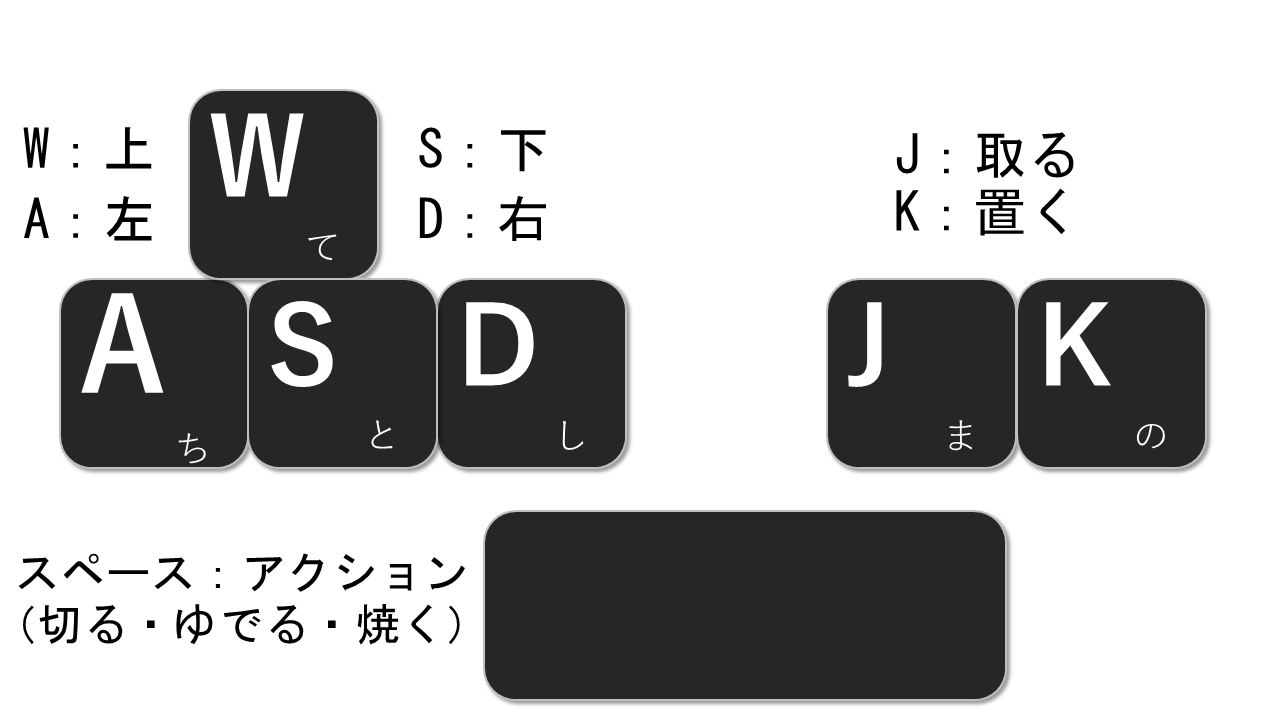
\includegraphics[scale=0.2]{img/key.png}
  \caption{キーボード操作方法}
  \end{center}
\end{figure}
\subsection*{(遊び方)}
\begin{enumerate}
  \item スタート\par
   スタートボタンを押すとゲームが開始する。 
  \item オーダーの確認\par
   まず、画面上部にランダムにオーダーが提示される。オーダーには、使う食材と調理方法が記載されている。各オーダーにはそれぞれ制限時間が設定されており、残り時間はオーダー上のゲージにリアルタイムに表示される。
  \item 食材の調理\par
   次に、オーダーに記載されている食材を、各食材ボックスから取り出す。各食材を持ったまま、各調理器具の前でアクションボタンを押すことで、食材が加工される。
  \item 料理の完成と提供\par
   料理は、加工された食材とお皿を組み合わせることで完成する。それらを組み合わせて料理ができあがれば、提供口に置くことで提供となり、オーダーと一致しているか判定される。一致していれば加点、間違っていれば減点となる。   
  \item リザルト\par
   制限時間がなくなるとリザルト画面に遷移する。スコアとランクが表示される。リザルトを押せばもう一度ゲームが開始する。
\end{enumerate}
\subsection*{(ゲーム画面)}
 ゲーム画面は図3のように、オーダー、キャラクター、食材・皿ボックス、スコア、調理器具、提供口、制限時間で構成されている。
\begin{figure}[H]
  \begin{center}
  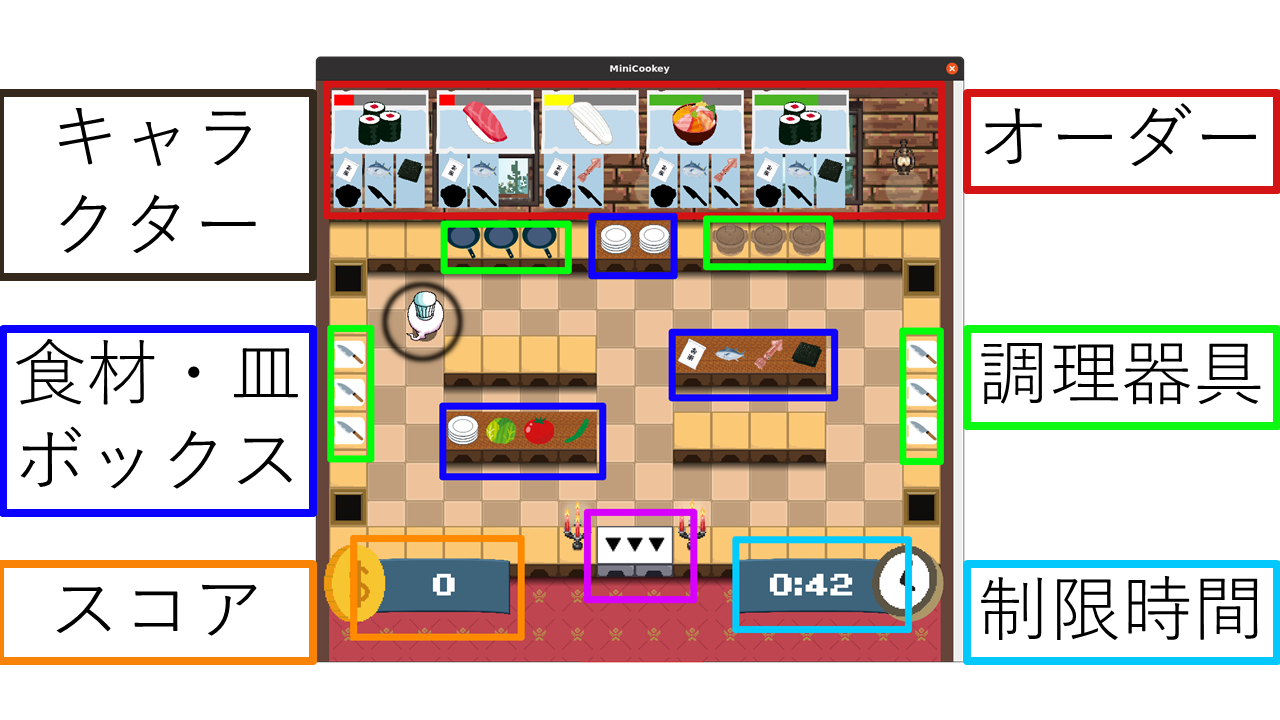
\includegraphics[scale=0.3]{img/game.png}
  \caption{ゲーム画面の説明}
  \end{center}
\end{figure}
\subsection*{(データ)}
\begin{itemize}
  \item メニュー一覧\par
    \begin{itemize}
      \item マグロ握り
      \item イカ握り
      \item 海鮮丼
      \item カッパ巻
      \item 鉄火巻き
      \item サラダ
    \end{itemize}
  \item 調理器具一覧\par
    \begin{itemize}
      \item 包丁
      \item 鍋
    \end{itemize}
  \item 食材一覧\par
    \begin{itemize}
      \item マグロ
      \item イカ
      \item 米
      \item 海苔
      \item キャベツ
      \item トマト
      \item キュウリ
    \end{itemize}     
\end{itemize}
文責:鈴木



\newpage
\section*{付録2:プログラムリスト}
以下にプログラムリスト全体を記述する。
\lstset{
    language=Java,
    inputencoding=utf8,
    %basicstyle=\ttfamily\scriptsize,
    basicstyle=\ttfamily\tiny,%最小文字、見にくいかも
    extendedchars=false,%日本語のためらしい
    breaklines=true,%長い行折る
    numbers=left,%行番号を左側に
    numberstyle=\tiny,%行番号サイズ
    stepnumber=1, %1行ごとに番号を表示
    frame=single, %枠
    tabsize=4 %タブの幅
}
\begin{itemize}
  \item MiniCook
  \lstinputlisting{../MiniCook.java}
  \item Model
  \lstinputlisting{../Model.java} 
  \item View
  \lstinputlisting{../View.java} 
  \item Controller
  \lstinputlisting{../Controller.java}  
  \item Order
  \lstinputlisting{../Order.java}
  \item Player
  \lstinputlisting{../Player.java}
  \item Start
  \lstinputlisting{../Start.java}
  \item Result
  \lstinputlisting{../Result.java}
  \item Meal
  \lstinputlisting{../Meal.java}
  \item Other
  \lstinputlisting{../Other.java}
  \item AudioManager
  \lstinputlisting{../AudioManager.java} 
\end{itemize}
\normalsize
文責:米谷・鈴木・吉田

\end{document}

\begin{comment}
\end{comment}